%%%%                %%%%
%%%% IMPLEMENTACIÓN %%%%
%%%%                %%%%

\chapter{Diseño e Implementación}
\label{chap:implemetación}

\lettrine{E}{ste} capítulo describe el diseño y la implementación de la solución construida. El sistema implementa un flujo de datos o pipeline. Toda la programación se ha realizado utilizando los lenguajes Python 3, C y Bash.

\section{Etapas del sistema}

Los datos son sometidos a un proceso por etapas tal como se ve en la Figura \ref{fig:vision-general-del-sistema}. A continuación se detalla cada una de estas etapas.

\begin{figure}[hp!]
    \centering
    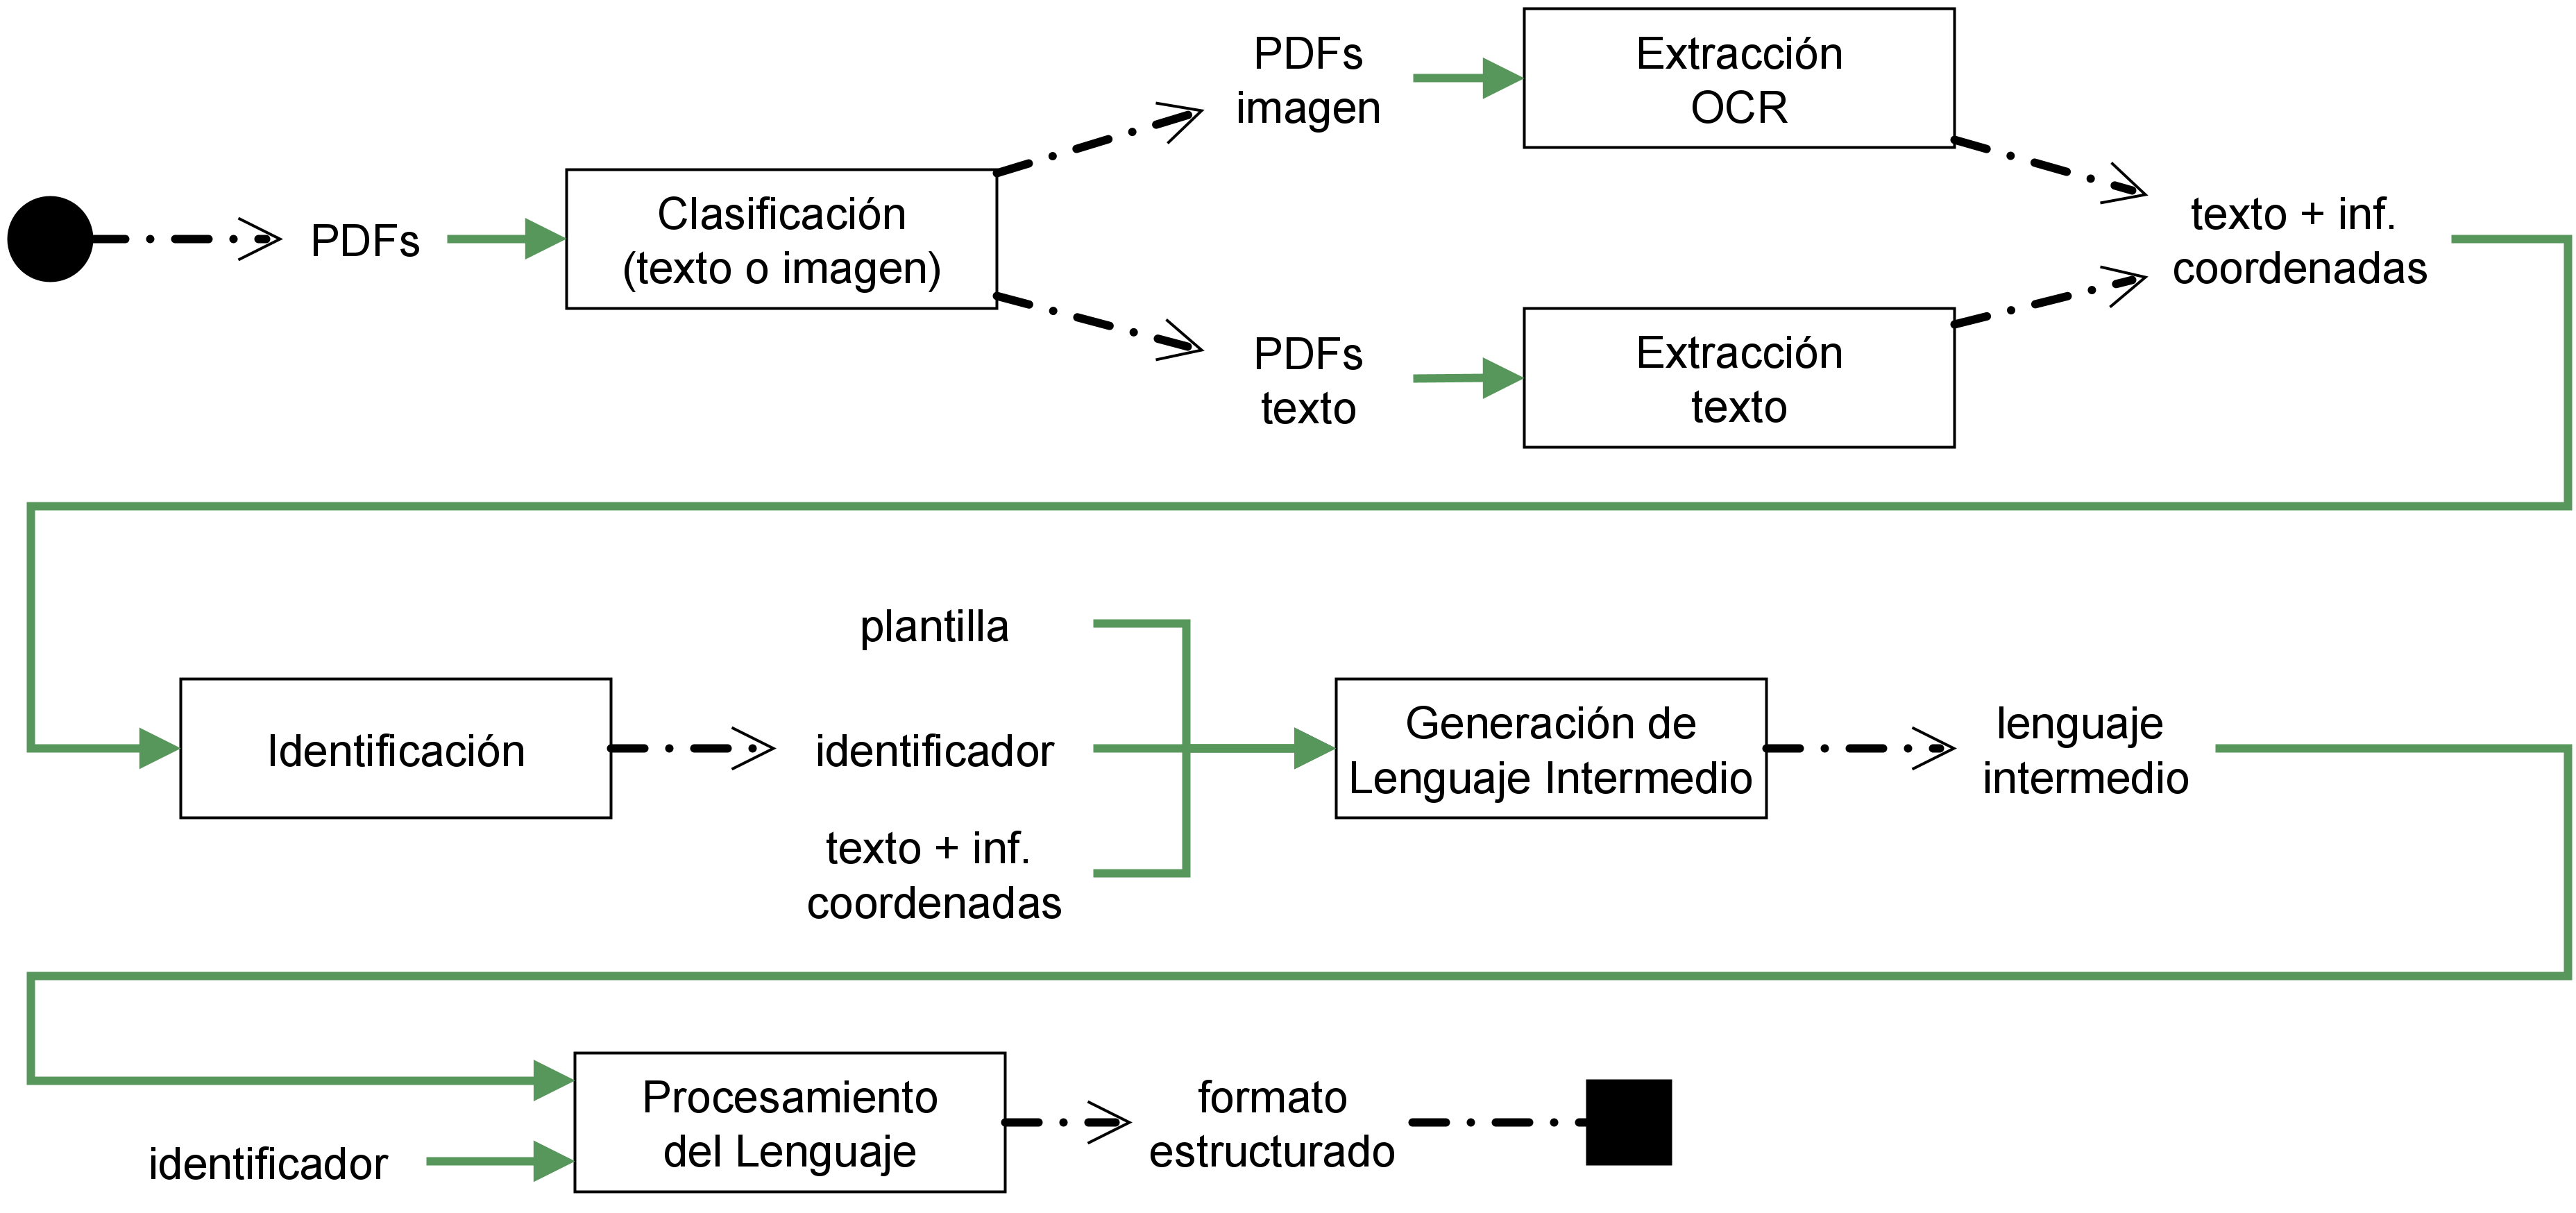
\includegraphics[width=1.0\textwidth]{imaxes/h-implementacion/vision-general-del-sistema-2}
    \caption{Visión general del pipeline del sistema}
    \label{fig:vision-general-del-sistema}
\end{figure}

El proceso comienza cuando se proporcionan al sistema un nuevo conjunto de ficheros PDF. La primera acción realiza la clasificación, según el tipo contenido de los PDF sean páginas con texto o con imágenes. El sistema mantiene el estado interno en base a la creación de los ficheros respetando un esquema de rutas particular.

A continuación se procede a la extracción de la información de los documentos. Además del propio texto, directamente visible, se genera la información de coordenadas que se utilizará para seleccionar los contenidos relevantes.

El proceso sigue con la identificación de los documentos con el objetivo de poder seleccionar la plantilla correcta, si está dada de alta en el sistema. 

Con toda la información obtenida se puede comenzar la generación del lenguaje intermedio de cada página. Para ello, la información de entrada está formada por la plantilla, el código del identificador encontrado y el texto con las coordenadas de la etapa de extracción.

Por último se transforma el lenguaje intermedio y se genera toda la información de salida del sistema. El identificador es utilizado en la  selección del parser necesario para transformar el documento. Cuando los procesos de análisis sintáctico han finalizado para los documentos, todos los datos de salida son movidos a un directorio de resultados y se genera la marca de finalización del tratamiento.

El componente referido como engine o motor se ocupa de conducir todas estas actividades, invocando uno a uno los scripts correspondientes a cada tarea y haciendo evolucionar el trabajo.

\subsection{Creación de un nuevo trabajo}

Si bien la Imagen \ref{fig:vision-general-del-sistema} representa el flujo de datos a nivel general, para comenzar el tratamiento se sigue un proceso formalizado en tres pasos. 

Primero el Sistema Externo solicita un identificador para el nuevo job. En ese momento el motor genera el código y lo utiliza para crear las rutas de directorios necesarias para ubicar los resultados de cada etapa. El identificador se obtiene de la fecha UTC actual concatenando segundos y nanosegundos. Se recurre al comando \verb|date| para ello, como se muestra en el Listado \ref{lst:creacion-job-id}.

\begin{lstlisting}[language=bash,caption={Obtención del identificador de un trabajo},label=lst:creacion-job-id]
job_id=$(date -u +%s%6N)
\end{lstlisting}

Utilizando el identificador, el Sistema Externo forma el path donde deberá depositar el fichero comprimido. Tras realizar la copia, se le debe indicar al motor que comience el procesamiento del trabajo para el identificador deseado.

% TODO valorar si incluir el comando de inicio de procesamiento

\subsection{Clasificación de los ficheros}

Como primera acción para tratar correctamente los ficheros se realiza un saneamiento de los nombres. Aplicar un nombrado homogéneo evitará problemas en la construcción de las rutas en el sistema de archivos. Para no perder la relación entre los nombres originales y los nuevos se crea en la ruta de salida un fichero para este dato con el el patrón <\#doc>.name. También se descartan los directorios que el fichero comprimido facilitado pudiera contener. El esquema de nombrado para los ficheros utiliza los números naturales comenzando en 1 y de forma creciente.

Los PDF recibidos deben ser clasificados dependiendo de su contenido. En unos casos es posible utilizar directamente el texto presenten en el documento. Para los restantes se procederá a utilizar el procedimiento OCR, como se ha explicado anteriormente. La clasificación se realiza por medio de un test de extracción de texto y se busca una respuesta positiva en la salida.

En \verb|extract-text.sh| se trata cada fichero PDF de tal manera que por cada uno se obtiene su número de páginas. La extracción de texto se realiza página a página, generando como salida un fichero individual para cada una. Desde este punto y para todos los demás procesos los documentos se tratan también página por página hasta llegar al procesamiento del lenguaje intermedio que recibe un único fichero para todas las páginas del documento. En el Listado \ref{lst:extraccion-text-inicial} se puede ver el cálculo del número de páginas y la instrucción de extracción.

\begin{lstlisting}[language=bash,caption={Extracción tentativa del texto},label=lst:extraccion-text-inicial]
last_page="$(pdfinfo $line | grep 'Pages:' | cut -c 7- | sed 's_ *__')"
for ((page=1; page<=$last_page; page++))
do
    pdftotext -f $page -l $page -layout "$line" "$n-$page_number.txt"
done
\end{lstlisting}

Cuando un documento no contiene texto, el fichero de la información extraída únicamente almacena caracteres de salto de página, \verb|0x0C|, que son introducidos por el propio \verb|pdftotext|. Estos casos pueden ser localizados mediante un editor hexadecimal, como se muestra en el Listado \ref{lst:deteccion-salto-pagina}. En el fragmento, tanto si se ejecuta el cuerpo del \verb|if| como del \verb|elif|, la página se trata de un caso de imagen y el fichero es movido al directorio para los casos de imagen.

\begin{lstlisting}[language=bash,caption={Detección del salto de página},label=lst:deteccion-salto-pagina]
if [ "$(hexdump -e '1/1 "%02X\n"' $i | tr '\n' ' ')" = '0C ' ]
then
    mv $i $base_image_dir
elif [ "$(hexdump -e '1/1 "%02X\n"' $i | tr '\n' ' ')" = '0C * ' ]
then
    mv $i $base_image_dir
fi
\end{lstlisting}

\subsection{Extracción de datos}

Previamente al proceso OCR, el script \verb|extract-images.sh| se encarga de extraer las imágenes contenidas en los ficheros seleccionados en el paso anterior. En este proceso se recupera la información original contenida en el PDF, no se trata simplemente de una captura de la página, sino que se utiliza la herramienta \verb|pdfimages| con el flag \verb|-j|. Si las imágenes presentes en el PDF fueron almacenadas en formato JPEG, con este flag se conseguirá recuperar la información sin realizar transformaciones y sin mayor pérdida de calidad, ya que el formato PDF soporta la codificación JPEG de forma nativa por medio de los filtros DCTDecode y JPXDecode \cite[23]{adobe_book_iso32000-1}. Además, al no requerir conversión la extracción es mucho más rápida. La situación descrita es la más habitual cuando un escáner profesional digitaliza un número de páginas y crea un PDF final para ellas.

El siguiente paso obtiene la información de coordenadas de los casos de texto, nuevamente con \verb|pdftotext|. Se generan los ficheros XHTML cuando se invoca la herramienta con el flag \verb|-bbox-layout|. En el Fragmento \ref{lst:extraccion-text-coord} se muestra un extracto del contenido típico que luego será procesado por el generador de código intermedio. Como se puede apreciar, se identifican la palabras individuales con coordenadas y la línea a la cual pertenecen.

\begin{lstlisting}[language=XML,caption={Extracción de texto con información de coordenadas},label=lst:extraccion-text-coord]
<flow>
    <block xMin="1594.583333" yMin="461.616667" 
            xMax="2148.275000" yMax="496.304167">
    <line xMin="1594.583333" yMin="461.616667" 
            xMax="2148.275000" yMax="496.304167">
        <word xMin="1594.583333" yMin="464.608333" xMax="1690.916667" 
                yMax="495.441667">Fecha</word>
        <word xMin="1748.350000" yMin="464.608333" xMax="1939.116667" 
                yMax="495.441667">facturación:</word>
    </line>
</block>
\end{lstlisting}

Completada la extracción de texto se da paso al proceso de OCR. El script \verb|image-apply-ocr.sh| recorre el directorio donde están almacenadas las imágenes recuperadas y se invoca a Tesseract con la instrucción que se puede ver en el Código \ref{lst:invocacion-de-tesseract}. Se indican varios parámetros importantes. Debe utilizar utilizar los conjuntos de entrenamiento para contenido en castellano (\verb|-l spa|), ya que los documentos están en este idioma. El número de \acrlong{ppp} se fija a 300 (\verb|--dpi 300|) ya que es es el tamaño mínimos que las imágenes deben tener para que el resultado del proceso OCR tenga calidad suficiente. Tesseract dispone de varios algoritmos para interpretar el layout de documento. En este caso, al trabajar directamente con las coordenadas, no es necesario tener en cuenta el layout y se le indica que capture la máxima información posible, independientemente del orden (\verb|--psm 11|). Por otra parte existe un fichero de configuración, apuntado por la variable \verb|$tessconfig_file| que contiene la directiva para activar la salida en formato hOCR, \verb|tessedit_create_hocr 1|.

\begin{lstlisting}[language=XML,caption={Invocación de Tesseract utilizada en el proyecto},label=lst:invocacion-de-tesseract]
tesseract $file_path "$outputbase" \
    -l spa \
    --dpi 300 \
    --psm 11 \
    -c page_separator='' \
    --tessdata-dir "$tessdata_dir" \
    $tessconfig_file
\end{lstlisting}

Se puede ver una muestra del formato hOCR en el Fragmento \ref{lst:salida-hocr-tesseract}. En el atributo \verb|title| de las palabras se puede ver que aparecen las coordenadas en píxeles respecto al tamaño de la imagen. También hay un indicador de confianza, \verb|x_wconf| que indica la certeza que asigna Tesseract a la correcta identificación de cada palabra en particular.

\begin{lstlisting}[language=XML,caption={Fragmento de la salida hOCR de Tesseract},label=lst:salida-hocr-tesseract]
<div class='ocr_page' id='page_1' 
    title='image "input/1627762529247627/based-image/1/1-000.jpg"; 
    bbox 0 0 2480 3509; ppageno 0'>
  <div class='ocr_carea' id='block_1_1' title="bbox 83 141 810 200">
    <p class='ocr_par' id='par_1_1' lang='spa' 
        title="bbox 83 141 810 200">
      <span class='ocr_line' id='line_1_1' title="bbox 83 141 810 200; 
          baseline 0.001 -16; x_size 59; 
          x_descenders 15; x_ascenders 15">
        <span class='ocrx_word' id='word_1_1' title='bbox 83 144 370 185; 
            x_wconf 96'>SALGADO</span>
        <span class='ocrx_word' id='word_1_2' title='bbox 390 141 701 200; 
            x_wconf 93'>Congelados,</span>
      </span>
\end{lstlisting}

\subsection{Identificación}
\label{subsec:impl-identificacion}
% TODO si se cambia implementación a SQLite, cambiar explicación.

Los documentos se identifican para poder asociarles una plantilla. El mecanismo utilizado consiste en buscar en la información extraída el dato que se ha considerado único para la familia de documentos. Para las facturas tratadas un dato único es el NIF o CIF del emisor, pero podría seleccionarse cualquier otros u otros, dependiendo del dominio. Los identificadores están almacenados en los ficheros \verb|id-nif-iva.txt| y \verb|id-cif.txt| en formato \acrshort{csv} en el directorio de datos del sistema.

El script \verb|identify-grep.sh| se encarga de realizar todo el proceso. Primero se leen todos los identificadores por medio de la función \verb|read_identifiers()|, tal como se puede ver en el Listado \ref{lst:lectura-de-identificadores}. Los datos leídos son incorporados a un array.

\begin{lstlisting}[language=bash,caption={Lectura de identificadores},label=lst:lectura-de-identificadores]
read_identifiers() {
    while IFS= read -r line; do
        # Add id if line has contents
        [ ! -z $line ] && ids_+=("$(echo -n $line | sed 's_._.*&_g' | cut -c 3-)")
    done < $1
}
\end{lstlisting}

A continuación se obtiene la lista de ficheros para los cuales se ha extraído información y se iteran buscando ocurrencias de los identificadores conocidos. En el Código \ref{lst:identifica-documentos} se le indica a \verb|grep| que tenga en cuenta solo los casos en los que el patrón abarque una palabra completa (\verb|-w|), y que cambie la salida habitual por otra con el recuento de ocurrencias (\verb|-c|).

\begin{lstlisting}[language=bash,caption={Identificación de los documentos},label=lst:identifica-documentos]
for file in $files; do
  for id_ in "${ids_[@]}"; do
    if [ "$(grep -w -c "$id_" $file)" -ge 1 ]; then
      #echo 'Found id: "'$id_'" in file: "'$file'"'
      echo $id_ | sed -E 's_\*|\.__g' > $dir_name/$number.id
      break
    fi
  done
done
\end{lstlisting}

Cuando se encuentra un identificador válido, se registra en el directorio del documento con un fichero que tiene por nombre el número del documento y la extensión \verb|id|. Por último se finaliza el bucle y se continúa con el siguiente documento.

\subsection{Plantillas y regiones}

% TODO completar significado de los campos que no son de coordenadas
% TODO is_global
% TODO page
% TODO doc_pages

Las plantillas contienen la información de coordenadas de las regiones de interés seleccionadas para el modelo de documento. En los ejemplos de Código \ref{comienzo-plantilla} y \ref{plantilla-ref-t1} se ver que para almacenar esta información se utiliza el formato JSON. Además de las coordenadas en si mismas, se utilizan otras claves para dar más flexibilidad a la información y poder tratar casos como los documentos de OVH. La clave \verb|id| que aparece al comienzo se utiliza para asociar con los identificadores de los documentos. Luego, el array \verb|regions| contiene la colección de regiones existentes en el modelo. Se utiliza \verb|type| para identificar el tipo de región, \verb|yMin| y \verb|yMax| para las coordenadas horizontales. Los límites verticales se almacenan en el array de columnas \verb|cols|. En el caso de regiones con una única columna, con el objetivo de mantener el formato homogéneo, se utiliza igualmente el array, pero con un único elemento.

\noindent\begin{minipage}{.45\textwidth}
    \begin{lstlisting}[language=Java,caption={Comienzo de la plantilla},label={comienzo-plantilla},frame=tlrb]{Name}
{
  "id": "A48941488",
  "is_global": false,
  "regions": [
    {
      "page": "0",
      "type": "R2",
      "doc_pages": "all",
      "yMin": 1112,
      "yMax": 1278,
      "cols": [
        {
          "xMin": 144,
          "xMax": 429
        },
        ...
    \end{lstlisting}
\end{minipage}\hfill
\begin{minipage}{.45\textwidth}
    \begin{lstlisting}[language=Java,caption={Región T1},label={plantilla-ref-t1},frame=tlrb]{Name}
    {
      "page": "0",
      "type": "T1",
      "doc_pages": "all",
      "yMin": 1281,
      "yMax": 2524,
      "cols": [
        {
          "xMin": 76,
          "xMax": 546
        },
        {
          "xMin": 860,
          "xMax": 1906
        }
        ...
    \end{lstlisting}
\end{minipage}

Es un formato aplicable para representar todas las regiones. Las coordenadas para las plantillas fueron creadas a mano durante el desarrollo utilizando el programa de edición de imágenes GIMP \footnote{\url{http://www.gimp.org.es/}}.

\subsection{Un engine modular}

% TODO Se imita un modelo de procesamiento en batch

El motor del sistema es el componente implementado en Bash. Esta decisión se tomó para facilitar el manejo de los ficheros dentro de la estructura de directorios. Además facilita el uso de herramientas en la shell, que sería más engorroso utilizar desde otros lenguajes de programación. 

\section{Generación del lenguaje intermedio}

La generación del lenguaje intermedio se realiza por medio de una aplicación Python escrita para este propósito. El código del programa está dividido en módulos de tal manera que se facilita el desarrollo y mantenimiento, agrupando lógica relacionada. La lista de módulos se presentan de forma resumida en la Tabla \ref{tab:modulo-generador-codigo-intermedio}.

Uno de los módulos comunes que se usa en toda la aplicación es \verb|constants.py|. Como evidencia su nombre, el objetivo del módulo es almacenar las constantes compartidas por todos los demás módulos. En particular, dado que se hace uso muy frecuente del tipo diccionario, todas las claves utilizadas se encuentran definidas en este fichero. En los listados de código se podrá apreciar que aparecen precedidas por el prefijo \verb|k| como en \verb|k_y_min|.

El lenguaje intermedio es suficientemente expresivo para representar los tipos de regiones, las filas, columnas de las tablas y las palabras. Al mismo tiempo evita complejidades que dificulten su tratamiento en los analizadores léxicos y sintácticos que se utilizan posteriormente. En la Imagen \ref{fig:lenguaje-intermedio} se presenta un extracto donde se puede observar la definición de tres regiones. La región \verb|T1| tiene tiene tres filas y tres columnas. La primera fila corresponde con la cabecera de la tabla. La elección de los símbolos para señalizar comienzo y fin de filas y columnas se escogió para hacer fácilmente reconocibles estos elementos al manejar los ficheros manualmente y no suponen especial complejidad en las reglas léxicas.

Las palabras siguen siempre el mismo patrón. Por ejemplo, en la caso \verb|P1·W146·365·| la primera parte, \verb|P1| indica la página del documento en donde se encuentra la palabra. \verb|W146| se refiere a que es una palabra del cuerpo, frente a una palabra de cabecera, que llevaría una \verb|H|. Por último \verb|365| es el contenido. Los demás símbolos se utilizan como separadores.

\begin{figure}[hp!]
    \centering
    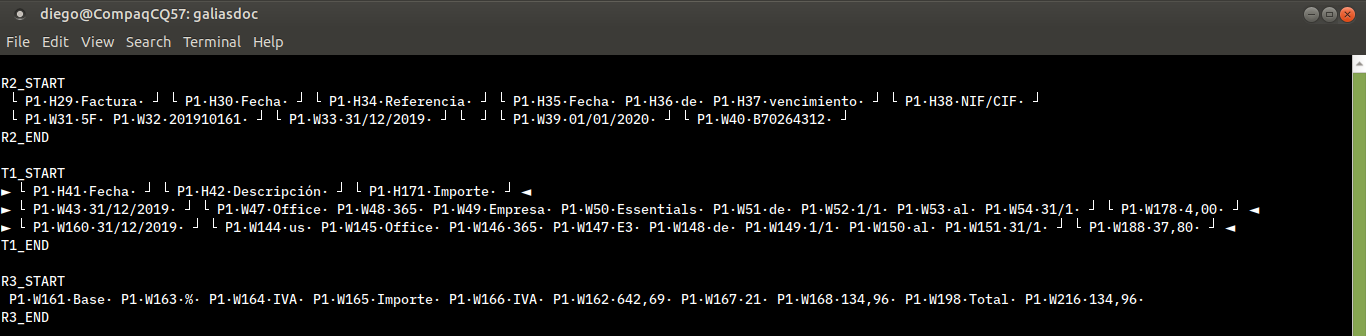
\includegraphics[width=1.0\textwidth]{imaxes/h-implementacion/lenguaje-intermedio.png}
    \caption{Extracto de lenguaje intermedio}
    \label{fig:lenguaje-intermedio}
\end{figure}

\begin{table}[ht]
    \centering
    \begin{tabular}{l l}
        Nombre del módulo & Objetivo \\
        \hline
        \hline
        assign.py & Asignación de líneas a regiones \\
        cli.py & Tratamiento de los argumentos de entrada \\
        constants.py & Almacén de constantes \\
        hough.py & Uso del algoritmo de Hough \\
        input\_handler.py & Parsing de los datos de entrada XHTML y hOCR \\
        lookup.py & funciones para búsqueda \\
        printer\_element.py & Funciones para la impresión de las palabras y líneas \\
        printer\_region.py & Funciones para la impresión de las regiones \\
        region.py & Tratamiento de las regiones \\
        task.py & Tareas definidas en la aplicación \\
        util.py & Utilidades comunes para toda el software \\
        main.py & Punto de entrada a la aplicación \\
    \end{tabular}
    \caption{Módulos del generador de lenguaje intermedio}    
    \label{tab:modulo-generador-codigo-intermedio}
\end{table}

Cuando se invoca la herramienta, el primer paso, además de realizar el tratamiento de argumentos de entrada, consiste en configurar la aplicación para que pueda generar la salida solicitada. En una ejecución interactiva, con el flag \verb|-h| se obtendrá ayuda sobre de los parámetros disponibles. En el Listado \ref{lst:ayuda-generador-codigo-intermedio} se puede ver este mensaje de ayuda y el significado de cada uno de los parámetros. Estos argumentos pueden ser de dos tipos, posicionales y opcionales. Los parámetros posicionales son obligatorios y deben ser indicados en el mismo orden que se muestra en la segunda línea del mensaje de ayuda. 

\begin{lstlisting}[caption={Ayuda del generador de código intermedio},label=lst:ayuda-generador-codigo-intermedio]
usage: main.py [-h] [-w WORKTASK]
parser_type text_with_coords template output_base number_pages page_image_path

positional arguments:
parser_type           Selecciona el tipo de parser HTML utilizado. Se puede
seleccionar entre HOCR y XML.
text_with_coords      Ruta al fichero del texto extraído/reconocido por OCR
con la información de coordenadas.
template              Ruta a la plantilla que ha de utilizarse con el
modelo.
output_base           Ruta base de salida para los ficheros generados
number_pages          Número de páginas del documento
page_image_path       Ruta a la imagen de la página

optional arguments:
-h, --help            show this help message and exit
-w WORKTASK, --worktask WORKTASK
Escoge el tipo de salida deseada. Por detecto produce la lista de palabras del fichero de entrada
\end{lstlisting}

El flag \verb|-w| se utiliza para escoger el tipo de salida que se desea. Seleccionando \verb|GENERATE| se obtiene el lenguaje intermedio. \verb|LIST_WORDS| produce un listado de todas las líneas y palabras asociadas. Mostrando por la salida estándar sus identificadores y coordenadas. Internamente estas tareas se definen como clases diferentes que exponen un método, \verb|run()|. Este método recibe los datos de la entrada y realiza el procesamiento de acuerdo a su objetivo. De esta manera es sencillo extender la aplicación para realizar distintos tipos de procesamientos.

El script \verb|generate-json.sh| es el encargado de realizar la invocación del generador de código intermedio con la parametrización necesaria para tratar cada página de forma individual.

La tarea de generación de código intermedio puede agruparse en los siguientes pasos, que se explicarán a continuación:

\begin{enumerate}
    \item Parsing de los datos en formato XHTML / hOCR
    \item Truncado de líneas y reasignación de líneas a regiones
    \item Tratamiento de las regiones
    \item Impresión del lenguaje
\end{enumerate}    

\subsection{Parsing de los datos}

Dado que ambos tipos de entradas tienen en común el formato (X)HTML, se utiliza el módulo \verb|HTMLParser| de la librería estándar Python para tratarlas. Se definen dos clases que extienden de \verb|HTMLParser| y sobrescriben los métodos \verb|__init__()|, \verb|handle_starttag()|, \verb|handle_data()| y \verb|handle_endtag()|. \verb|handle_starttag()| y \verb|handle_endtag()| son llamados cuando el parser encuentra el comienzo y final de un tag, respectivamente. \verb|handle_data()| es invocado para tratar los datos de la etiqueta, en este caso interesa el contenido de las palabra y la ocurrencia de las líneas.

\noindent\begin{minipage}{.45\textwidth}
    \begin{lstlisting}[language=Python,caption=Captura de las palabras,frame=tlrb,label={lst:captura-de-palabras}]{CapturaDePalabras}
def handle_data(self, data):
  if self.store_word == True and 
      data.strip() != '':
    self.lines[-1][k_words].append(
        self.word_counter)
    self.words.append({
        k_id: self.word_counter,
        k_value: data,
        k_x_min: self.wxMin,
        k_y_min: self.wyMin,
        k_x_max: self.wxMax,
        k_y_max: self.wyMax})
    \end{lstlisting}
\end{minipage}\hfill
\begin{minipage}{.45\textwidth}
    \begin{lstlisting}[language=Python,caption=Recuperación de coordenadas,frame=tlrb,label={lst:recuperacion-coordenadas}]{RecuperacionCoordenadas}
def get_coords(self, attrs):
    xMin = int(float(attrs[0][1]))
    yMin = int(float(attrs[1][1]))
    xMax = int(float(attrs[2][1]))
    yMax = int(float(attrs[3][1]))
    return xMin, yMin, xMax, yMax
    \end{lstlisting}
\end{minipage}

En el Listado \ref{lst:captura-de-palabras} se puede como se utiliza una lista donde se almacenan estructuras de tipo diccionario para todos los datos de una palabra. Las coordenadas se recuperaron previamente leyendo los atributos en el método de apertura, tal como se muestra en el Listado \ref{lst:recuperacion-coordenadas}. También se utiliza un contador para generar los identificadores de las palabras en la variable \verb|self.word_counter|. Por último, al almacenar las líneas, se les asocian las palabras que contienen por medio de los identificadores descritos. 

\subsection{Truncado de líneas y reasignación de líneas a regiones}

Una vez leída la información, se tienen en memoria todas las líneas y palabras con sus posiciones. El siguiente paso consiste en asignar las líneas a las regiones que les corresponden atendiendo a las coordenadas de ambas.

Para asociar líneas o palabras las regiones definidas en las plantillas se utiliza un algoritmo genérico. Es genérico ya que compara dos regiones rectangulares y resuelve si una está sobre la otra, en base a sus coordenadas y dimensiones. Este algoritmo se utiliza en varios punto del programa para clasificar líneas en regiones o líneas en columnas de las regiones.

Al comienzo del desarrollo se realizó una primera implementación para resolver esta clasificación pero utilizaba Sets de Python como tipo de dato y resultaba excesivamente lenta. Con la aproximación actual se comparan nueve casos. Si hay dos rectángulos, $ \alpha $ y $ \beta $ y se quiere saber $ \alpha $ está dentro de $ \beta $, primero se comprueba si, atendiendo a sus coordenadas, está totalmente dentro. Este es un caso muy frecuente. En los demás se mira si $ \alpha $ podría estar sobre alguno de los lados de $ \beta $ y por último si $ \alpha $ podría estar en alguna sobre alguna de las esquinas de $ \beta $. Una representación gráfica de los casos puede verse en la Imagen \ref{fig:casos-algoritmo-seleccion-regiones} del Apéndice. 

Los datos de entrada son la lista de áreas que se quieren clasificar y la zona sobre la que se quiere realizar el test. Un bucle recorre las áreas evaluando los criterios. La asignación de un área a la zona se produce si todas las condiciones son verdaderas en alguno de los casos. Para considerar las situaciones donde $ \alpha $ está sobre el borde de $ \beta $, se tiene en cuenta un margen de proximidad, configurado para el $ 30\% $. Con esto se regula cuanto puede sobresalir $ \alpha $ de $ \beta $ para seguir siendo considerada válida para el caso. En el Listado \ref{lst:condiciones-caso-b} se puede ver el código donde se evalúan las condiciones para ser perteneciente al caso B mostrado en \ref{fig:casos-algoritmo-seleccion-regiones}.

\begin{lstlisting}[language=Python,caption={Evaluación de las condiciones del Caso B},label=lst:condiciones-caso-b]
    case_b = [element[k_x_max] > container[k_x_min],
    element[k_x_max] <= container[k_x_max],
    element[k_y_min] >= container[k_y_min],
    element[k_y_max] <= container[k_y_max],
    element[k_x_min] < container[k_x_min],
    container[k_x_min] - element[k_x_min] < x_length]
\end{lstlisting}

El truncado de líneas resuelve un problema descubierto durante el desarrollo y que no había sido considerado previamente. La longitud de las líneas identificadas por los procesos de extracción excede frecuentemente el tamaño de las columnas definidas en las plantillas. A la hora de generar el lenguaje hay que colocar las palabras en una única columnas de las tablas. Por tal motivo, es necesario truncar las líneas y crear otras nuevas que encajen dentro de las columnas y reasignar las palabras a las nuevas columnas. En la Imagen \ref{fig:visor-formato-hocr} del Apéndice se puede ver, por ejemplo, que los datos correspondientes a la tarifa y al IVA, están en la misma zona verde, la misma línea. Esto quiere decir que para el formato hOCR o \verb|pdftotext| una línea se asimila como una secuencia de caracteres próximos, y no como todo el contenido de una fila de la tabla o una línea de una página de texto.

% TODO detalle del algoritmo de truncado

\subsection{Tratamiento de las regiones}

El tratamiento de las regiones comienza seleccionando aquellas que aplican a la página. El parámetro \verb|page| que cada región tiene definida en las plantillas especifica si la región a de ser considerada para la página teniendo en cuenta el número de página actual y el total de páginas del documento. El parámetro se evalúa como un \emph{slice} Python y da suficiente flexibilidad para todos los casos que se han encontrado hasta el momento. En el Listado \ref{lst:seleccion-de-regiones-segun-pagina} se muestran ejemplos de uso en una sesión interactiva. La implementación hace uso del método \verb|eval()| para la evaluar expresiones a partir de literales: \verb|eval(f"doc_page_numbers[{region_slice}]")| donde \verb|doc_page_numbers| es la lista con los números de las páginas, que se generó previamente.

\begin{lstlisting}[language=Python,caption={Selección de regiones según las páginas},label=lst:seleccion-de-regiones-segun-pagina]
Python 3.6.9 (default, Jan 26 2021, 15:33:00) [GCC 8.4.0] on linux
Type "help", "copyright", "credits" or "license" for more information.
>>>
>>> paginas = list(range(1,11)) # lista de páginas
>>> paginas
[1, 2, 3, 4, 5, 6, 7, 8, 9, 10]
>>> paginas[0] # solo aplica a la primera página
1
>>> paginas[-1] # solo a la última
10
>>> paginas[-1] # a todas las páginas
[1, 2, 3, 4, 5, 6, 7, 8, 9, 10]
>>> paginas[1:-1] # todas menos primera y última
[2, 3, 4, 5, 6, 7, 8, 9]
\end{lstlisting}

Una vez seleccionadas las regiones se procede a procesarlas. En el módulo \verb|region.py| existe una clase para cada una de ellas. La mayoría definen únicamente un método, \verb|assign_lines()| y también el constructor, para inicializar la clase con las coordenadas de la región. Si la región tienen columnas, se informa también de las posiciones de las mismas. El objetivo de método \verb|assign_lines()| es recorrer las columnas, o el espacio principal si no hay columnas y llamar a \verb|assign_words_to_regions_geometric()| con cada una de ellas. El método anterior corresponde al algoritmo genérico de clasificación de regiones comentado en la Subsección anterior. Una responsabilidad más de \verb|assign_lines()| es guardar, junto con los demás datos de la región, la implementación necesaria para crear el texto de salida. Lo que se hace es asignar directamente la referencia a alguno de los métodos del módulo \verb|printer_region.py|. Las funciones de impresión se comentarán más adelante, pero es en este punto cuando se realiza la selección, dado que cada tipo de región genera un texto diferente.

Estas clases descritas están diseñadas para ser genéricas, no estando asociadas a ningún tipo de modelo en particular. En el caso de los documentos de OVH se crearon unas regiones diferentes, \verb|T2_T2_R1|, por ejemplo, ya las regiones que están contiguas unas a otras indican como se han de asignar los datos. A pesar de ello, nada limita que cualquiera de ellas se pueda aplicar en el futuro a otros modelos de documentos que compartan las mismas características.

\subsection{Impresión del lenguaje}

En este punto se han asignado las líneas a las regiones que les corresponde. En el módulo \verb|printer_region.py| se encuentran las funciones que toman la regiones, líneas y palabras y crean el texto que finalmente se escribirá a disco. Por ejemplo, en la implementación para las tablas T1, los pasos que se siguen consisten en buscar todas las líneas \emph{reales} de la tabla. Por líneas reales se entienden aquellas que forman una unidad de contenido, independientemente de cuantas líneas físicas tenga dicho contenido. Para ello se toman como referencia las líneas de la primera columna. Estas líneas se comparan en altura con todas las demás que están en la tabla. Para ser consideradas al mismo nivel, la altura debe ser la misma, aceptando un margen del $ 25\% $ de desviación. Este porcentaje es el que mejor resultados ofreció en las pruebas. A continuación se trasladan a la primera línea todas las palabras que están en segundas líneas físicas. Por último, solo queda recorrer las líneas, columnas y palabras acumulando el string generado y que se corresponde con el lenguaje intermedio.

La escritura en disco se realiza una vez el flujo a llegado de vuelta a la tarea GENERATE, donde además se imprimen los ficheros de líneas y palabras que se listan en la Tabla \ref{tab:datos-de-salida}.

% TODO información de bounding box
% TODO explicar se utiliza el algoritmo de Hough en los ejemplos donde es efectivo

Por último, en la Tabla \ref{tab:datos-intermedios} se presenta la relación de ficheros existentes para un documento cuando la generación del lenguaje intermedio finaliza. Estos datos no se exportan a al directorio de salida. En la tabla se muestran tanto los ficheros para casos de imagen como de texto.

\begin{table}[ht]
    \centering
    \begin{tabular}{l l}
        Esquema del nombre del fichero & Contenido \\
        \hline
        \hline
        \verb|<#doc>-<#pag>-language.txt| & Lenguaje intermedio para una página \\
        \verb|<#doc>-<#pag>.box| & Lista carácter a carácter y coordenadas (Tesseract) \\
        \verb|<#doc-<#pag>.hocr| & Dados en formato hOCR (Tesseract) \\
        \verb|<#doc>-xxx-language.txt| & Documento global del lenguaje intermedio \\
        \verb|<#doc>.id| & Identificador de la plantilla \\
        \verb|<#doc>-<#pag>.xml| & XML resultado de la extracción de texto \\
        \verb|<#doc>-<#pag>.txt| & Texto obtenido de \verb|pdftotext| \\
    \end{tabular}
    \caption{Resumen de los datos de salida}    
    \label{tab:datos-intermedios}
\end{table}

\section{Procesamiento del lenguaje intermedio}

% Diferencias organizativas
La organización de la aplicación a nivel código fuente en esta parte del proyecto presenta diferencias respecto a los que sería un programa clásico hecho en Flex y Bison, tal y como se presenta en la Subsección \ref{subsec:flex}. En caso de proceder del modo tradicional, las reglas de distintos modelos estaría todas en el mismo fichero, que crecería con cada nuevo modelo a tratar. Además, organizar las reglas para evitar colisiones supondría un alto coste de mantenimiento. Se hacía necesario encontrar un aproximación más flexible para permitir que con un mismo ejecutable fuese posible iniciar múltiples analizadores léxicos y sintácticos. Una alternativa que se barajó fue la de crear un ejecutable por cada modelo, aplicaciones independientes, pero se descartó por ser excesivamente compleja y poco elegante. En la aproximación utilizada, cada modelo de documento tienen su par de ficheros \verb|.y| y \verb|.l|, que son totalmente independientes a otros ficheros de reglas. No solo eso, además, la compilación también es independiente. Se puede considerar que cada modelo se implementa como un plugin al sistema.

En el Listado \ref{lst:fuentes-del-procesador-de-lenguajes} del Apéndice se pueden ver todos los ficheros fuente que forman parte del procesador de lenguaje. Alternativamente, en la Tabla \ref{tab:modulos-procesador-lenguaje} están relacionados los más relevantes.

\begin{table}[ht]
    \centering
    \begin{tabular}{l l}
        Módulo & Responsabilidades \\
        \hline
        \hline
        \multicolumn{2}{c}{tool-parser/main/ ↓} \\
        \hline    
        \verb|main.c| & Inicializaciones, argumentos de entrada, carga e invocación del parser \\
        \verb|app-conf.h| & Tipos de datos para la configuración de la aplicación \\
        \verb|gen.c| & Generación de tablas de datos y palabras seleccionadas \\
        \verb|get-amounts.c| & Generación de importes \\
        \verb|global-vars.h| & Definiciones de variables globales para usar en Bison \\
        \verb|types.h| & Estructuras de datos para la fase generación \\
        \verb|flex-prologue.{c,h}| & Prólogo Flex único \\
        \verb|bison-prologue.{c,h}| & Prólogo Bison único \\
        \verb|bison-epilogue.{c,h}| & Epílogo Bison único \\
        \hline
        \multicolumn{2}{c}{tool-parser/plugin/ ↓} \\            
        \hline        
        \verb|*.l| & Fuentes Flex para todos los modelos \\
        \verb|*.y| & Fuentes Bison para todos los modelos \\
        \hline
        \multicolumn{2}{c}{tool-parser/lib/ ↓} \\     
        \hline
        \verb|util.c| & Utilidades para toda la aplicación \\
    \end{tabular}
    \caption{Módulos de procesador de lenguaje}    
    \label{tab:modulos-procesador-lenguaje}
\end{table}

\subsection{Carga dinámica del parser}

Definiendo el include de \verb|dlfcn.h| en un programa C se tienen acceso a las funciones que permiten realizar la carga dinámica de ficheros \verb|.so| y la ejecución de una función cuyo prototipo sea conocido de antemano. En este caso, primero se define el puntero a función que se necesita:

\begin{lstlisting}[language=C,caption={},label={}]
int (*parse)();
\end{lstlisting}

Luego se realiza la apertura de la librería dinámica que se quiere utilizar, pero no se cargan en memoria los símbolos que contiene. La inicialización es lazy:

\begin{lstlisting}[language=C,caption={},label={}]
handle = dlopen(app_config->plugin_path, RTLD_LAZY);
\end{lstlisting}

Se obtiene la dirección de memoria del símbolo que se quiere utilizar, en este caso la función \verb|yyparse()|. Esta función la define Bison:

\begin{lstlisting}[language=C,caption={},label={}]
parse = dlsym(handle, PARSER_NAME);
\end{lstlisting}

Y por último se ejecuta el parser a través del puntero a función. Cuando el proceso finaliza correctamente la variable \verb|completed| valdrá 0. En caso de valer 1, lo más habitual es que se produjese un error de sintáctico en el parser:

\begin{lstlisting}[language=C,caption={},label={}]
int completed = (*parse)();
\end{lstlisting}

Para finalizar se cierra la librería compartida y, en este caso, también en fichero de entrada.

\begin{lstlisting}[language=C,caption={},label={}]
dlclose(handle);
fclose(yyin);
\end{lstlisting}

\subsection{Dependencias entre módulos}

Al tener una colección de parsers, las secciones de los prólogos y el epílogo de Bison tienen partes comunes en todos los casos. Para evitar redundancias y seguir la propuesta del principio de diseño DRY, se crearon módulos específicos para albergar todo aquello que es común a todos los parsers y se realiza su inclusión previamente a cualquier otro contenido. Haciéndolo así, los analizadores no pierden las secciones sino que estas contienen únicamente las definiciones específicas para tratar cada una las particularidades de su modelo. La relación de dependencias puede verse en las Figuras \ref{fig:dependencia-flex} y \ref{fig:dependencia-bison}

\begin{figure}
    \centering
    \begin{subfigure}[b]{0.40\textwidth}
        \centering
        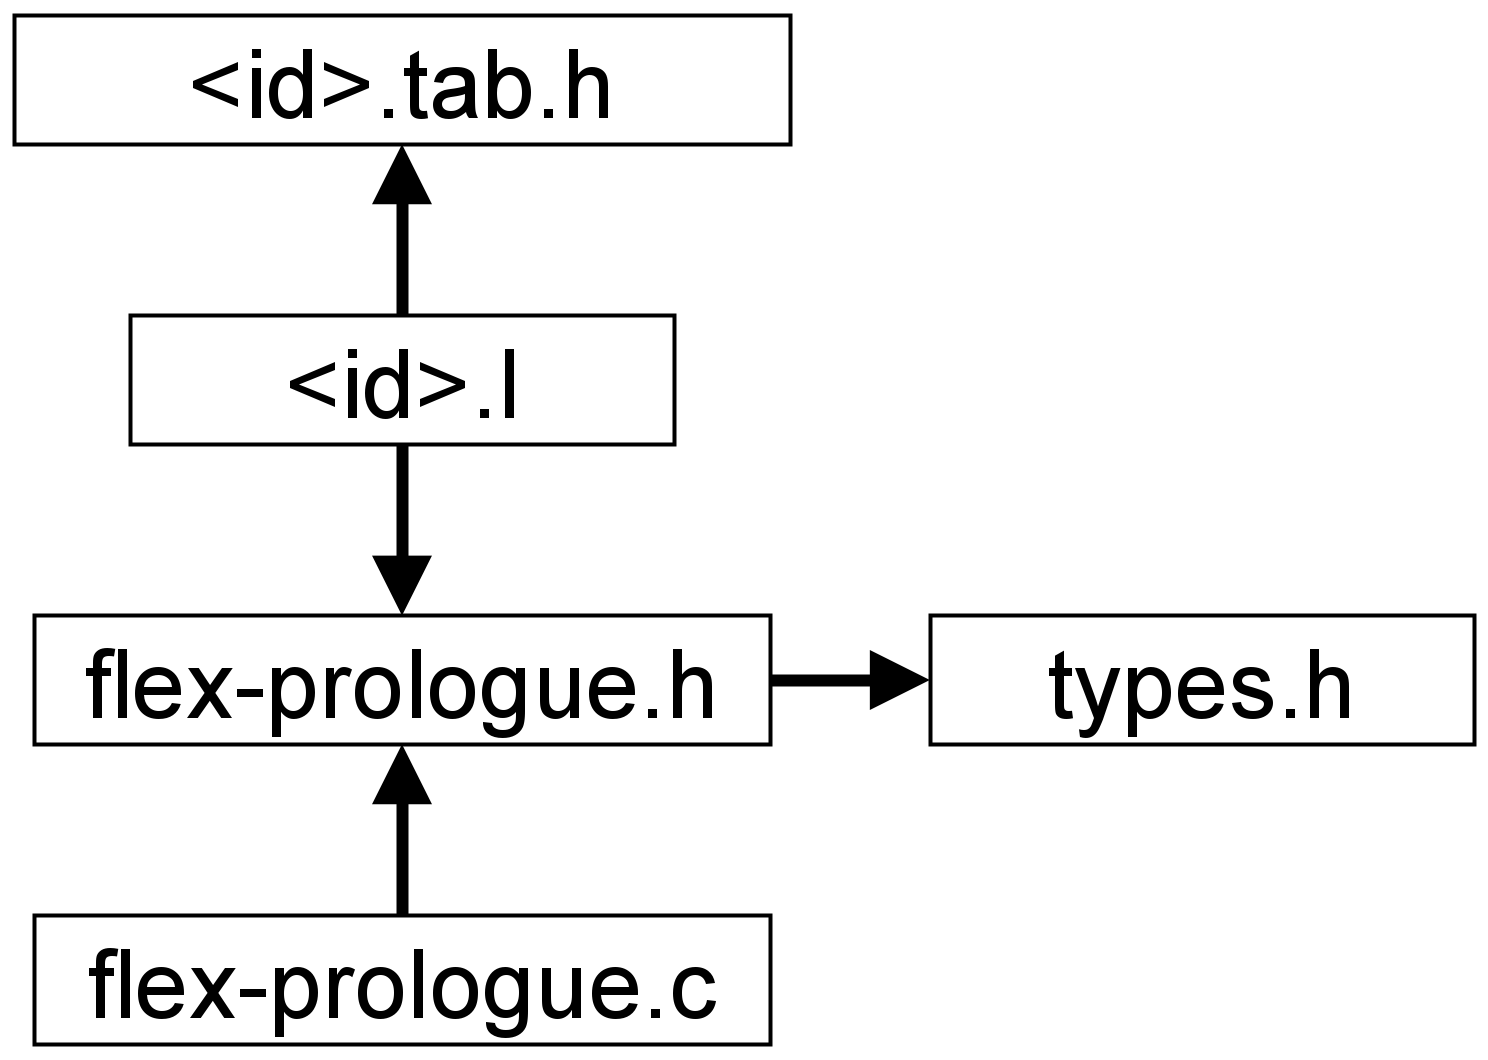
\includegraphics[width=\textwidth]{imaxes/h-implementacion/relaciones-flex}
        \caption{Dependencias Flex}
        \label{fig:dependencia-flex}
    \end{subfigure}
    \hfill
    \begin{subfigure}[b]{0.59\textwidth}
        \centering
        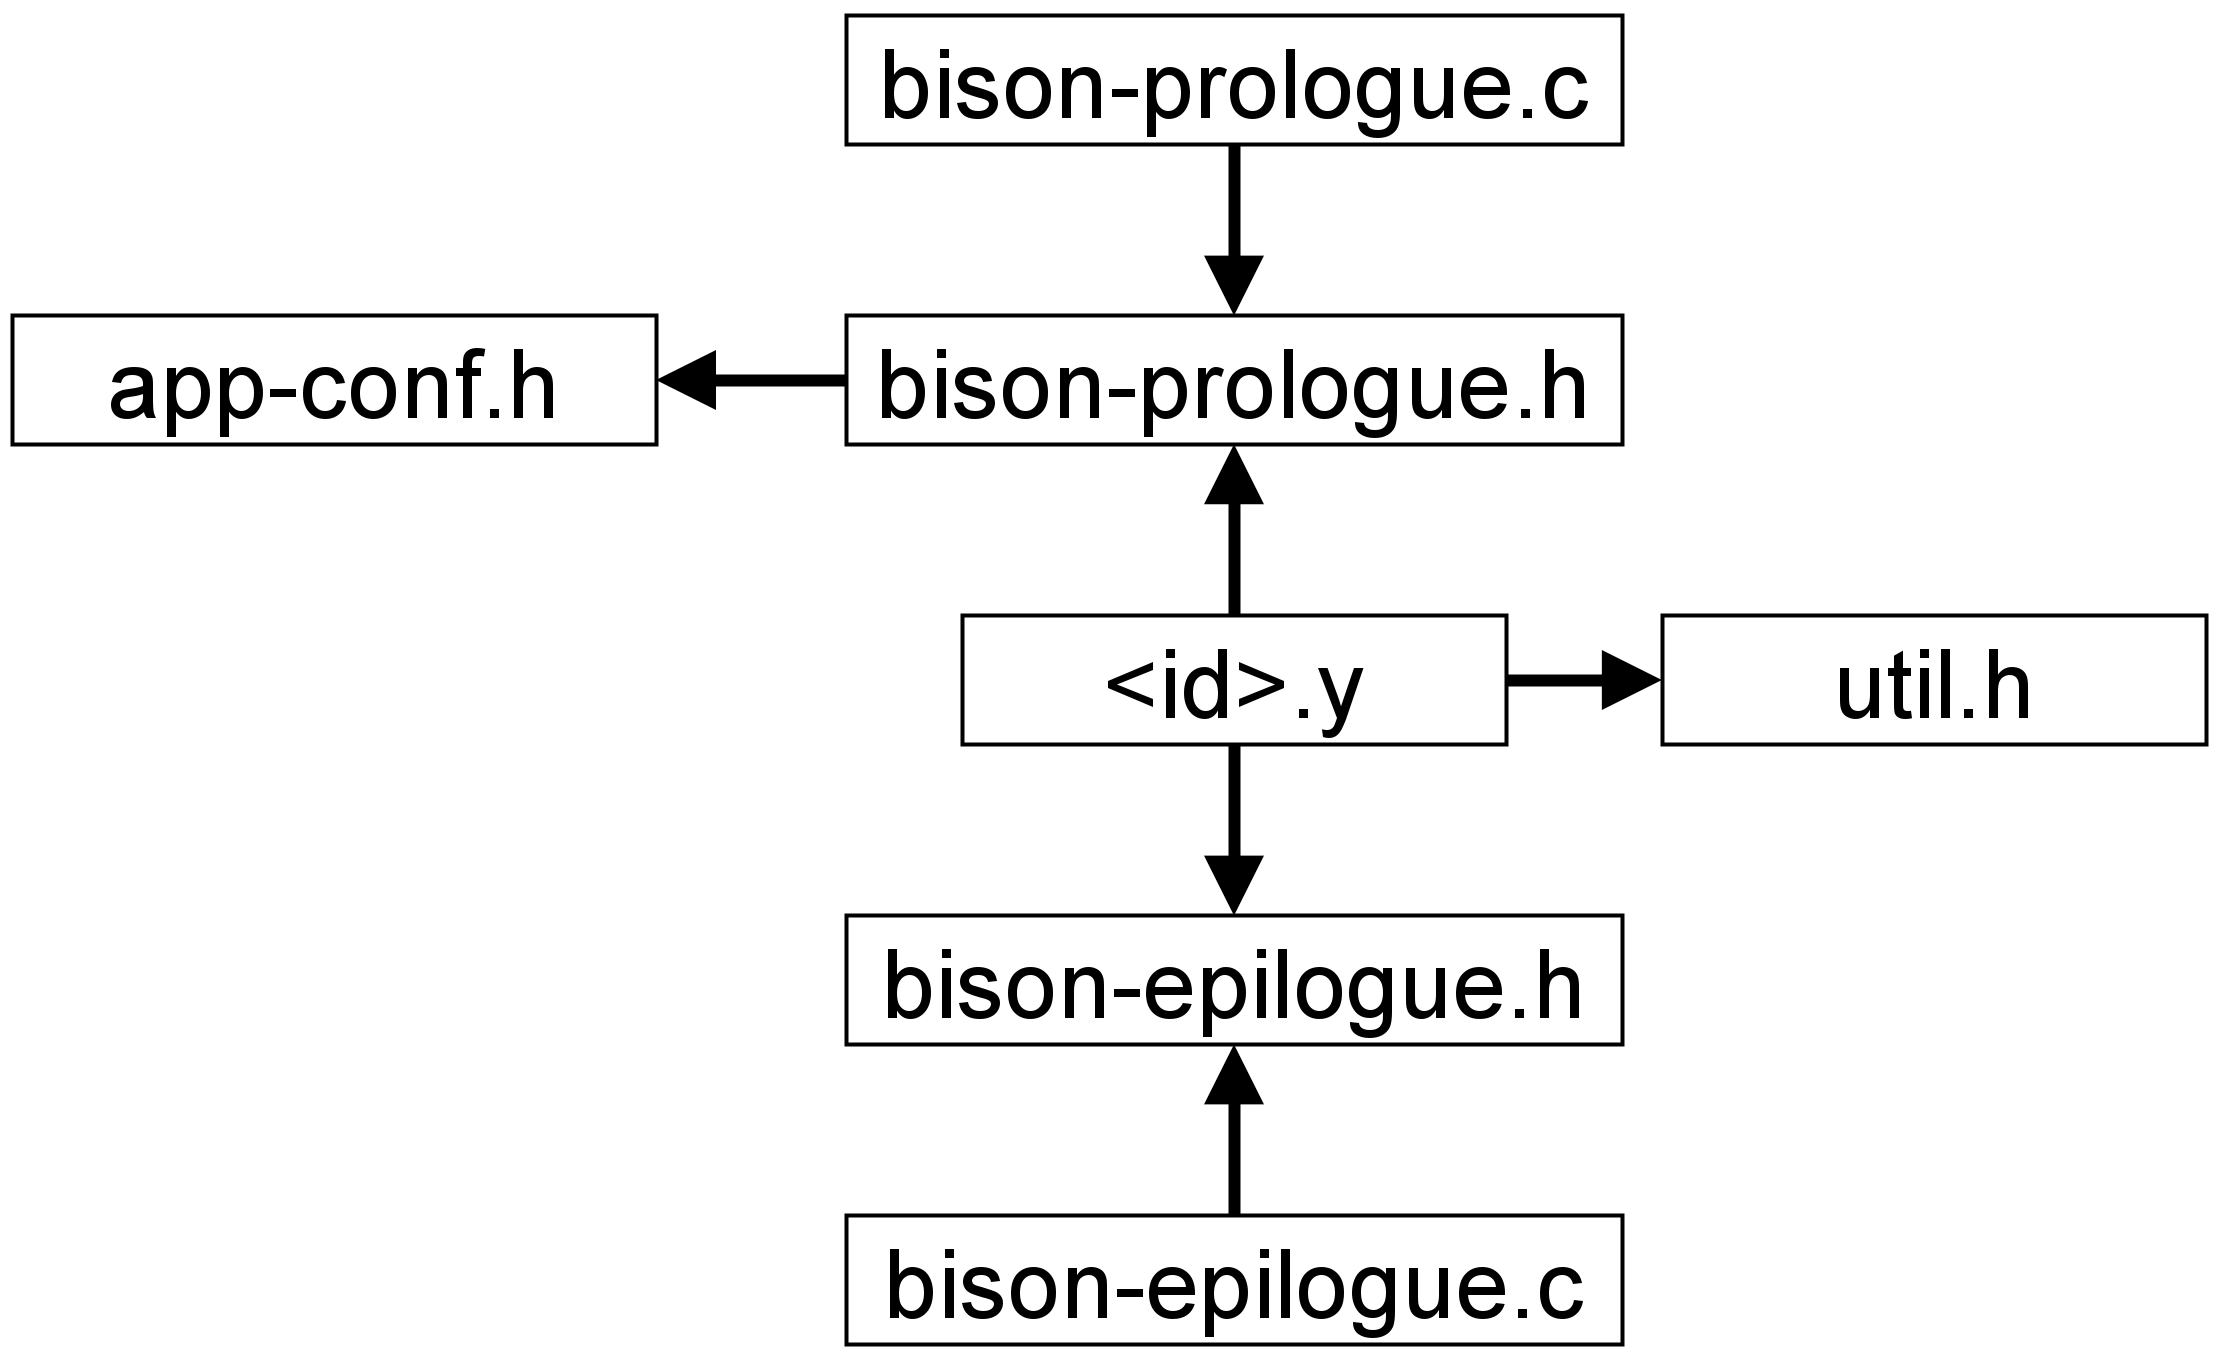
\includegraphics[width=\textwidth]{imaxes/h-implementacion/relaciones-bison}
        \caption{Dependencias Bison}
        \label{fig:dependencia-bison}
    \end{subfigure}
\end{figure}

Por ejemplo, en \verb|flex-prologue.c| se puede encontrar la implementación de la función \verb|split_id_value| (el prototipo completo es \verb| word_value *split_id_value(char *contents)|) cuyo cometido es recibir una palabra como, \verb|P1·W146·365·|, dividirla en componentes y crear su representación en memoria. El tipo de dato definido para las palabras es un \verb|struct| y se puede encontrar en \verb|types.h|:

\noindent\begin{minipage}{.45\textwidth}
    \begin{lstlisting}[language=C,caption={},frame=tlrb,label={}]{}
typedef struct word {
    char *value;
    char *w_id_string;
    int w_id_numeric;
    \end{lstlisting}
\end{minipage}\hfill
\begin{minipage}{.45\textwidth}
    \begin{lstlisting}[language=C,caption={},frame=tlrb,label={}]{}
    int w_id_numeric;
    char *w_page_number_string;
    int w_page_number_numeric;
} word_value;
    \end{lstlisting}
\end{minipage}

Para evitar la necesidad de conversiones de tipos en cualquier otro punto del programa, los identificadores se guardan como strings, lo que resulta útil durante escritura en disco, y también como enteros, en el caso de necesitar realizar cualquier operación con ellos.

El fichero \verb|bison-prologue.h| contiene las definiciones de prototipos de \verb|yyerror()| e \verb|yylex()|, que son llamadas durante la ejecución de \verb|yyparse()|. \verb|yylex()| es la función para ejecutar el escáner. \verb|yyerror()|, que se define en \verb|bison-epilogue.c| tienen por finalidad mostrar los errores del tratamiento por la salida de error, \verb|stderr|.

\subsection{Variables globales}

Debido a la reestructuración, las variables que se definen en el epílogo de Bison no están disponibles durante el parseo. El epílogo es donde está normalmente la función \verb|main()|. Aquí la función \verb|main()| es totalmente independiente y tienen su módulo propio. Esto es un inconveniente debido a que hay información necesaria que no va a ser accesible fuera del \verb|main()|. Por ejemplo, los parámetros de entrada al programa, que son tres:

\begin{itemize}
    \item La ruta al fichero del lenguaje intermedio.
    \item La ruta al fichero del identificador del documento (el fichero \verb|.id|).
    \item Y la ruta al plugin, para poder realizar la carga dinámica.
\end{itemize}

El path del fichero del lenguaje intermedio se descompone en partes (ruta de salida, número de documento) y se utilizan en la fase de generación para escribir los ficheros de resultados en la ruta y con el nombre correctos. Para la generación de los datos de las tablas en formato CSV no se utiliza el \acrshort{ast} sino que se utiliza una lista donde se guardan únicamente los datos relacionados con un tipo de dato para este caso.

El acceso a esta información no es posible si no se emplean variables globales. El \verb|struct app_config| disponible en el módulo de cabecera \verb|app-conf.h| contiene los tipos de datos para guardar toda la información relativa a los parámetros de entrada y cualquier otro dato de configuración que fuese necesario. En el módulo \verb|global-vars.h| están las declaraciones de las variables que contendrán los datos de importes.

\subsection{Compilación separada}

La obtención los ejecutables se automatiza con GNU Make y dado que la carga de los parsers se realiza como librerías dinámicas, la compilación se puede llevar a cabo de forma separada ya que los parsers no se enlazan con el programa principal. Para su distribución, es posible crear versiones que contengan algunos parsers y no otros.
Para la obtención de las librerías dinámicas se compilan primero los módulos dependientes de los que se ha hablado anteriormente, prólogos y epílogo, y también los módulos utilizados en la fase de generación. En las líneas de Código de ejemplo la variable $ \$@ $, propia de Make, contiene el nombre del fichero que se va a compilar:

\begin{lstlisting}[language=C,caption={},label={}]
gcc -fPIC -c $@.c
\end{lstlisting}

El parámetro \verb|fPIC| de GCC compila los módulos de manera que el código generado no depende de estar en una dirección de memoria específica para funcionar y es necesario para el correcto funcionamiento de las librerías dinámicas. A continuación ya se puede compilar cada uno de los parsers:

\begin{lstlisting}[language=C,caption={},label={}]
bison -y -Wno-yacc -d -r all -o $(PLUGIN)/$@.tab.c $(PLUGIN)/$@.y
flex -o $(PLUGIN)/$@.yy.c $(PLUGIN)/$@.l
gcc -fPIC -c $(PLUGIN)/$@.tab.c
gcc -fPIC -c $(PLUGIN)/$@.yy.c
gcc -o $@.so -shared bison-epilogue.o flex-prologue.o $@.tab.o $@.yy.o
\end{lstlisting}

Las dos primeras líneas generan los analizadores sintáctico y léxico, respectivamente. Se hace en este orden para poder incluir el fichero \verb|*.tab.c| en el analizador léxico. Este fichero es generado por Bison contiene y contiene, por ejemplo, las definiciones de tokens compartidas por ambos. En la quinta línea se compila la librería y se obtiene el fichero \verb|.so|.

\subsection{Análisis léxico}

Cuando se invoca la función \verb|yyparse()| comienza el análisis sintáctico para el modelo cargado. En esta fase se utilizan tanto tipos de datos definidos en \verb|types.h| como otros desarrollados por terceros. 

El árbol de parseo se almacena como un tipo abstracto lista. Algunos de los elementos del árbol, si son recursivos, utilizan a su vez otras listas. Estas relaciones continúan hasta llegar las variables que contienen las palabras. La implementación del tipo de datos lista se encuentra en los módulos \verb|lista.{c,h}| y contiene todos los métodos habituales para la creación y liberación de listas e inserción, obtención y borrado de elementos. 

En el programa, para la manipulación de strings se recurre a funciones de la librería estándar de C como, \verb|strdup()|, pero también se utiliza el tipo de dato \verb|strbuf|, que expone sus métodos en el módulo de cabecera \verb|strbuf.h|. Este módulo tiene operaciones seguras para actuar sobre cadenas. Los \verb|strbuf| se pueden concatenar, copiar y formatear, de igual forma a como se utiliza en \verb|printf()|.

Tanto \verb|lista.c| como \verb|strbuf| han sido desarrolladas por terceros y no forma parte del trabajo realizado para este TFG.

Para almacenar los tipos de regiones se creó el tipo \verb|region| como un \verb|struct| compuesto de un enumerado y un \verb|union|. Cuando se crea una nueva región le asigna un tipo del enumerado y se utiliza para los datos la variable correspondiente del \verb|union|. Más tarde en la generación, se sigue el mismo mecanismo para recuperar los datos de la lista o tabla correcta:

\noindent\begin{minipage}{.45\textwidth}
    \begin{lstlisting}[language=C,caption={},frame=tlrb,label={}]{}
typedef struct region {
    enum {
        R_R1,
        R_R2,
        R_R3,
        R_T1,
        R_T2
    } type;
    \end{lstlisting}
\end{minipage}\hfill
\begin{minipage}{.45\textwidth}
    \begin{lstlisting}[language=C,caption={},frame=tlrb,label={}]{}
    union {
        lista r1;
        lista r2;
        lista r3;
        table t1;
        table t2;
    };
} region;
    \end{lstlisting}
\end{minipage}

La tablas se almacenan en un \verb|struct| que contiene dos listas, una para las palabras de la cabecera y otra para las filas de la tabla. A su vez, las columnas son listas con palabras:

\noindent\begin{minipage}{.45\textwidth}
    \begin{lstlisting}[language=C,caption={},frame=tlrb,label={}]{}
typedef struct table {
    lista col_titles;
    lista rows;
} table;
    \end{lstlisting}
\end{minipage}\hfill
\begin{minipage}{.45\textwidth}
    \begin{lstlisting}[language=C,caption={},frame=tlrb,label={}]{}
typedef lista cols;
    \end{lstlisting}
\end{minipage}

Los ficheros de reglas Flex tienen similitudes en lo que se refiere a los tokens para los delimitadores de las regiones y las palabras. En el Listado \ref{lst:reglas-lexicas} se pueden ver reglas disponibles. Las dos primeras líneas encuentras los delimitadores para el tipo de región T1. En este caso no es necesario ningún valor semántico. La tercera regla corresponde a una palabra de una cabecera (lleva \verb|H| en lugar de \verb|W|). La última regla se utiliza para encontrar las palabras que forman el contenido. Nótese que aquí si se devuelve un valor semántico por medio de la variable \verb|yylval.word_value|. Además se define en la regla una función útil si se necesita depurar el escáner. La activación de esta función se controla por medio del flag \verb|-DDEBUG_LEXER| del preprocesador de C. De tal manera que si este flag no se indica, la función no está presente en el código generado.

\begin{lstlisting}[language=C,caption={Reglas léxicas habituales},label={lst:reglas-lexicas}]
"T1_START" {return T1_START;}
"T1_END" {return T1_END;}
"P"{number}"·H"{number}"·Importe·" {return IMPORTE;}
"P"{number}"·W"{number}"·"{word}"·" {
    PRINTF("WORD[\%s]\n", yytext); yylval.word_value = split_id_value(yytext);
    return WORD; }
\end{lstlisting}

\verb|word| y \verb|number| son expresiones regulares definidas en la sección de definiciones con la finalidad de ser reutilizables.

\begin{lstlisting}[caption={Expresiones regulares para palabras y números},label={lst:word-and-number}]
word [\ 0-9A-Za-zÁÉÍÓÚÑáéíóúñ\.\,\-\$\%&\*\?\(\)\"\_\:\'\/\|\+]+
number [0-9]+
\end{lstlisting}

Otra responsabilidad de los analizadores léxicos es limpiar los datos recibidos. Las palabras Tarifa e IVA del documento de AC que se muestra en el la Imagen \ref{fig:visor-formato-hocr} del Apéndice llegan juntas en el lenguaje intermedio ubicadas en la columna del IVA. La forma recibida es \verb|P1·W134·32,240010,00·|. El 10 y los dos decimales a la derecha deben separarse y habilitar un mecanismo para poder colocar el dato de la tarifa en su columna. En este caso se genera un token específico, \verb|DOUBLE_WORD| para que el analizador sintáctico pueda tratarlo.

\subsection{Análisis sintáctico}

Aunque las reglas se analizan en Bison desde las hojas al axioma, para facilitar la exposición se mostrarán de forma inversa, mostrando aquellas que son comunes a todos los parsers.

El axioma es equivalente a una lista de regiones y en la acción se llama a las dos funciones de generación, \verb|gen_contents()| y \verb|gen_table_amounts()|. Cuando el flujo retorna a la acción después de la generación, se llama a una última función, \verb|free_ast()| cuyo cometido es la liberación de la memoria reservada para el \acrshort{ast}.

Las regiones almacenan en el árbol mediante dos reglas, la primera de ellas recursiva:

\begin{lstlisting}[caption={},label={}]
regions: regions region  {
    $$ = $1;
    lista_append(&$$, $2);
} | region {
    nueva_lista(&$$);
    lista_append(&$$, $1); }
\end{lstlisting}

La recursividad sucede porque el no terminal resultado, \verb|regions|, aparece también en la parte derecha de la primera regla. Se utiliza recursividad por la izquierda, según se recomienda en el manual de Bison para mantener el uso del espacio del stack acotado. En caso de utilizar recursividad por la derecha, el espacio utilizado es proporcional al número de elementos de la secuencia, que necesitan ser movidos a la pila antes de que la regla pueda ser aplicada.

Cuando llega la primera región se produce una reducción por la segunda de las reglas. En ese momento se inicializa la lista de regiones, accesible en la variable \verb|$$|, y se  guarda la región actual accediendo al valor semántico de su no terminal, \verb|$1|. Para las sucesivas regiones aplica la primera regla, que tiene que conservar el puntero a la lista y guardar la región desde el segundo no terminal.

Descendiendo un nivel están las reglas para formar las regiones. En este punto se inicializa el \verb|struct region|, asignándose el tipo correspondiente:

\begin{lstlisting}[caption={},label={lst:guardando-regiones}]
region: t1 {$$->type = R_T1;, $$->t1.rows = $1;} | r3 {$$->type = R_R3;}
\end{lstlisting}

En las reglas donde están disponibles los datos económicos de las facturas, estos se guardan también en la variable global \verb|table_amounts_|:

\begin{lstlisting}[caption={},label={}]
word_value *word_total = lista_get($2, 2);
table_amounts_->total = word_total;
\end{lstlisting}

Las líneas de las tablas son otra estructura recursiva que opera de manera similar al caso de las regiones. Y ocurre de igual manera con las columnas y las palabras.

La regla para el token \verb|WORD| pasa los datos al no terminal \verb|word| y además se utiliza para encontrar el mayor número de página dentro del documento. Este dato se utiliza en la generación pero no se recibe como parámetro ya que se puede calcular a partir de las propias palabras. Solo es necesario actualizar el dato en \verb|app_config_->max_page_number|.

Una característica de Bison no comentada es que tanto los terminales como los no terminales pueden tener un tipo de dato asociado, si es necesario, para trasladar un valor semántico hacia arriba en el árbol de parseo. En la sección de definiciones se pueden encontrar todos los terminales y no terminales conocidos para el parser y los tipos asignados, Listado \ref{lst:definiciones-tipos-bison}. Para poder subir información por el árbol, todos los símbolos de la gramática deben tener el dato correcto.

\noindent\begin{minipage}{.45\textwidth}
    \begin{lstlisting}[language=C,caption={Definiciones de tipos para tokens y no terminales},frame=tlrb,label={lst:definiciones-tipos-bison}]{}
%token TOTAL TIPO
%token <word_value> WORD
%type<region> region
%type<word_value> word
%type<lista> line lines r3 regions
    \end{lstlisting}
\end{minipage}\hfill
\begin{minipage}{.45\textwidth}
    \begin{lstlisting}[language=C,caption={Tipo de variables compartidas entre Bison y Flex},frame=tlrb,label={lst:union-variables-compartidas}]{}
%union {
    int *int_pointer;
    char *string;
    lista lista;
    region *region;
    word_value *word_value; }
    \end{lstlisting}
\end{minipage}

Para que la información semántica pueda ser compartida entre Bison y Flex, en Bison se define la variable \verb|yylval| a la que Flex tiene acceso. Esta variable contiene un \verb|union| de C que se configura en el analizador sintáctico, un ejemplo de tipos utilizados puede verse en el Listado \ref{lst:union-variables-compartidas}.

\subsection{Generación de código}

La fase de generación de código o, en este caso, creación de los distintos ficheros de salida, se realiza recorriendo el \acrshort{ast} y seleccionando los datos necesarios. La función \verb|gen_contents()| dirige todos los pasos. Primero se genera el JSON \footnote{Para crear las salidas en formato JSON se utiliza la librería cJSON de Dave Gamble que está disponible en Github, \url{https://github.com/DaveGamble/cJSON}.} con los tipos de palabras seleccionadas y después el CSV de la tabla de datos. Las funciones que tratan cada tipo de región comparten todas un mismo prototipo. Como se generan dos tipos de salida, existe una función para cada región y cada tipo de salida. Este modelo obliga a realizar dos recorridos sobre el árbol, pero simplifica la programación ya que cada función se centra únicamente el los datos que necesita para su salida en particular.

La definición de las funciones se hace por medio de un array estático de punteros a función, como se muestra en el Listado \ref{lst:def-estaticas-funciones-regiones}. La variable \verb|fa| del array (linea 7) selecciona la columna del mapa \verb|GENERATION_MAP| que corresponde para las funciones que tratan la selección de palabras, en el caso mostrado. Existe otro array análogo que contiene los punteros a las funciones de la última columna.

\begin{lstlisting}[caption={Definiciones estáticas para las funciones que tratan las regiones},label={lst:def-estaticas-funciones-regiones}]
#define GENERATION_MAP(X) \
/* Region type, Handlers selected words,   Handlers XML contents */ \
X(R_R1,         handler_selected_words_r1, handler_xml_contents_r1) \
X(R_T2,         handler_selected_words_t2, handler_xml_contents_t2)

handler handlers_selected_words[] = {
    #define X(op, fa, fb) [op] = fa,
    GENERATION_MAP(X)
    #undef X };
\end{lstlisting}

Por último solo queda recorrer la lista de regiones invocando a al método necesarios con el array: 

\begin{lstlisting}[caption={},label={}]
    for (int i = 0; i < regions.len; i++) {
        region *region = lista_get(regions, i);
        if (NULL != handler_array[region->type]) {
            handler_array[region->type](region, contents); } }
\end{lstlisting}

En el caso de la generación del CSV para la tabla de datos, existe una función común para las regiones T1 y T2. Al tratar la región es necesario recorrer las filas y columnas. El texto del CSV se concatena en un \verb|strbuf| que se devuelve para su escritura a disco.

% TODO generación de las palabras selecconadasd

% TODO generación de la tabla CSV

% TODO generación de los importes

% TODO Mostrar como se utiliza la librería para generación de ficheros JSON

\subsection{Salida generada}

La Tabla \ref{tab:datos-de-salida} presenta un resumen de los datos que se obtienen como salida del proceso. Todos los ficheros relativos a un documentos llevarán prefijado en número del documento y el número de la página individual, donde sea necesario.

\begin{table}[ht]
    \centering
    \begin{tabular}{l l}
        Esquema del nombre del fichero & Contenido \\
        \hline
        \hline
        \verb|<#doc>-<#pag>-lines.json| & Líneas de la página, ubicaciones y palabras asociadas \\
        \verb|<#doc>-<#pag>-selected.json| & Palabras de la página seleccionadas como relevantes \\
        \verb|<#doc>-<#pag>-words.json| & Todas las palabras del documento y sus ubicaciones \\
        \verb|<#doc>.jpg| & Imagen de la página \\
        \verb|<#doc>-amounts.json| & Importes totales e individuales obtenidos de las tablas \\
        \verb|<#doc>-table.csv| & Datos de la tabla de datos principal \\
        \verb|<#doc>.name| & Nombre original del fichero PDF\\
    \end{tabular}
    \caption{Resumen de los datos de salida}    
    \label{tab:datos-de-salida}
\end{table}

\section{Despliegue}

Inicialmente no se pensó en Docker para el proyecto. Si se deseaba disponer de algún mecanismo para automatizar los deployments \footnote{Se entiende por deployment todas aquellas actividades necesarias para que un software esté disponible para su uso en un entorno de producción.} y para ello se seleccionó Ansible, con el que se desarrolló un script inicial. A raíz de las adaptaciones para la construcción del prototipo surgió la necesidad de ejecutar la aplicación en un entorno Windows. Aunque algunas de las herramientas utilizadas en el proyecto están disponibles en este sistema operativo, por ejemplo a través de Cygwin \footnote{\url{https://www.cygwin.com/}}, tanto el rendimiento como la disponibilidad de todos los paquetes era incierta. Además de otros posibles problemas que pudieran surgir, como el tratamiento de paths en Windows vs. Linux. Docker proporciona una solución apropiada en este escenario.

\subsection{Docker}

Para \emph{Dockerizar} un aplicación se necesita escribir un \verb|Dockerfile|. Este fichero está en la raíz del proyecto. Las sentencias del \verb|Dockerfile| se ejecutan en secuencia para construir la imagen Docker de la aplicación. Una imagen, en este contexto, es el conjunto de instrucciones que permiten a Docker crear un contenedor. Las imágenes se forman a partir de capas de software superpuestas y cuando una capa cambia, también se reconstruyen las superiores. En este caso se utiliza como base Ubuntu 18.04, indicado en el fichero con la instrucción \verb|FROM ubuntu:bionic|. Sobre ella se crean las capas adicionales por medio de varias instrucciones \verb|RUN|. Con ellas se lleva a cabo \footnote{Ver Apéndice, Sección \ref{sec:instalacion-software} para más detalles del repositorio y los paquetes.}:

\begin{enumerate}
    \item El alta del repositorio de Tesseract actualizado.
    \item Se instalan todas las dependencias para la ejecución de la aplicación.
    \item Se instalan paquetes para la compilación en C (\verb|build-essential|, por ejemplo).
    \item Se copia el proyecto a una carpeta dentro de la imagen.
	\item Con \verb|RUN make -C galiasdoc| se compila la aplicación. Donde \verb|-C| indica a Make que cambie al directorio \verb|galiasdoc| y luego ejecute el target \verb|all| en él. Tras la compilación se exporta el directorio de distribución, \verb|dist|, que contiene todos los ficheros necesarios para la ejecución.	
\end{enumerate}

% TODO Mostrar fichero de configuración Docker y su uso

% TODO valorar si comentar como Docker construye imágenes en capas del software

% TODO valorar si incluir capítulo o sección de pruebas. O, al menos, de pruebas realizadas.
